 \documentclass[conference]{IEEEtran}

\usepackage[spanish]{babel}
\usepackage[utf8]{inputenc}
\usepackage{graphicx}
\usepackage[hidelinks]{hyperref}
\usepackage{xurl}
\usepackage{microtype}
\usepackage{enumitem}
\usepackage{tikz}
\usetikzlibrary{positioning,arrows.meta}

\begin{document}

\title{Informe de Computación Científica con Python\\
\Large Consecuencias de la Inteligencia Artificial en las personas}

\author{\IEEEauthorblockN{Martín Arrigo}
\IEEEauthorblockA{\textit{Instituto de Informática} \\
\textit{Universidad Austral de Chile}\\
Valdivia, Chile \\
martin.arrigo@alumnos.uach.cl}

\and
\IEEEauthorblockN{Nicolás Toro}
\IEEEauthorblockA{\textit{Instituto de Informática} \\
\textit{Universidad Austral de Chile}\\
Valdivia, Chile \\
nicolas.toro@alumnos.uach.cl}
\\[1cm]
\IEEEauthorblockN{Diego Mora}
\IEEEauthorblockA{\textit{Instituto de Informática} \\
\textit{Universidad Austral de Chile}\\
Valdivia, Chile \\
diego.mora01@alumnos.uach.cl}
\and
\IEEEauthorblockN{Benjamín Neira}
\IEEEauthorblockA{\textit{Instituto de Informática} \\
\textit{Universidad Austral de Chile}\\
Valdivia, Chile \\
benjamin.neira@alumnos.uach.cl}}

\maketitle

\let\thefootnote\relax\footnotetext{Profesor: Luis Veas. Año: 2026.}

\begin{abstract}
Este informe presenta un análisis descriptivo sobre las consecuencias de la Inteligencia Artificial (IA) en las personas. A partir de varios conjuntos de datos filtrados, se evalúan dimensiones clave como la salud mental, el impacto en el empleo y las percepciones sociales sobre privacidad y seguridad. El análisis incluye la relación entre la percepción de reemplazo laboral y el nivel de agotamiento (\textit{burnout}) en diversos profesionales, así como las actitudes del público frente a la adopción de la IA y sus riesgos inherentes. Los resultados preliminares muestran tendencias significativas, como un mayor agotamiento asociado al temor de automatización en ciertos roles tecnológicos, y cómo la confianza en la herramienta moldea la percepción social de beneficio o amenaza.
\end{abstract}

\begin{IEEEkeywords}
inteligencia artificial, consecuencias sociales, salud mental, privacidad, seguridad, educación, empleo.
\end{IEEEkeywords}

\section{Introducción}
La expansión de herramientas de IA está modificando la forma en que las personas estudian, trabajan, se informan y toman decisiones [5-6,8-9]. Sin embargo, existe incertidumbre sobre sus efectos concretos en la vida cotidiana y sobre qué grupos enfrentan mayores riesgos o beneficios.

Aunque la IA se ha difundido rápidamente, su adopción no ocurre de manera homogénea entre personas y contextos. Factores como edad, nivel educativo y entorno laboral pueden condicionar tanto la intensidad de uso como la percepción de beneficios y riesgos. Por ello, analizar el fenómeno únicamente desde promedios generales puede ocultar diferencias relevantes para una interpretación social más precisa.

Para evitar sesgos derivados de datos agregados, este trabajo prioriza registros crudos y comparables. En educación, la evidencia muestra que modelos como ChatGPT ya alcanzan alto rendimiento en pruebas universitarias, ubicandose en el percentil 91 para Microeconomía y el percentil 99 para Macroeconomía en comparación con los estudiantes que toman el examen TUCE al final de su curso de principios. Los resultados muestran que ChatGPT es capaz de proporcionar respuestas que superan las respuestas medias de los estudiantes, generando desafíos para la integridad académica [5]. En privacidad y seguridad, se han identificado riesgos de desinformación, filtraciones y usos maliciosos de los modelos de lenguaje [6]. En empleo y productividad, estudios recientes estiman una exposición significativa de tareas a la automatización y mejoras de productividad con asistencia generativa [7-8], en línea con proyecciones institucionales sobre cambios en ocupaciones y habilidades [9].

En este trabajo se procederá a realizar un análisis descriptivo y comparativo con el objetivo de responder a las siguientes preguntas iniciales:
\begin{enumerate}
\item ¿Cómo se asocian burnout, satisfacción laboral y reemplazo de tareas con la intensidad de uso de IA en el trabajo?
\item ¿Qué percepciones de confianza y beneficio sobre la IA predominan en la sociedad?
\item ¿Cómo interactúa el nivel de confianza en la IA con la percepción de amenaza a las libertades individuales o el apoyo a regulaciones éticas?
\item ¿De qué manera incide el uso de IA y el nivel de dependencia en el rendimiento académico de los estudiantes?
\item ¿Cómo se distribuye geográficamente el desarrollo de Inteligencia Artificial?
\end{enumerate}

Para abordar estas preguntas, utilizaremos distintos gráficos con el fin de visualizar de forma más clara los datos obtenidos y facilitar una mejor comprensión de sus patrones, tendencias y posibles contrastes entre grupos.

\section{Solución propuesta}
La solución propuesta consiste en un pipeline de análisis preliminar en Python con tres etapas:

\begin{enumerate}
\item Integración y limpieza de los tres datasets principales (Data\_set\_01, Data\_set\_02 y Data\_set\_03), ademas de datos obtenidos apartir de un crawler que recopila informacion de la ocde desde el año 2022 al 2024.
\item Armonización de variables por dimensión del problema (salud mental, privacidad/seguridad, productividad/empleo y educación).
\item Generación de gráficos preliminares para observar tendencias y formular hipótesis de investigación.
\item Generación de mapas geográficos para visualizar la distribución del desarrollo de IA a nivel global.

\end{enumerate}

Esta solución permite responder de forma inicial las preguntas planteadas en la introducción y deja preparado el terreno para análisis posteriores con técnicas inferenciales.

\section{Metodología y procesamiento en Python}
El procesamiento se realizó en Python con \texttt{pandas} y \texttt{numpy} para limpieza y agregación, y \texttt{matplotlib}/\texttt{seaborn} para visualización. El flujo aplicado fue:
\begin{itemize}
    \item Carga de los CSV y revisión de estructura, tipos de datos y valores nulos.
    \item Tratamiento de nulos en variables de uso de IA.
    \item Construcción de variables derivadas (por ejemplo, Uso de IA) y normalización simple por grupos cuando corresponde.
    \item Generación de gráficos directamente en Jupyter para el análisis descriptivo.
\end{itemize}

\section{Diagrama del problema en estudio y dimensiones}
\begin{figure}[!htbp]
\centering
\begin{tikzpicture}[scale=0.6, transform shape,
    box/.style={draw, align=center, font=\small, minimum width=24mm, minimum height=7mm},
    smallbox/.style={draw, align=center, font=\small, minimum width=24mm, minimum height=6mm},
    arrow/.style={-Latex, thick}
]
% Nodos principales (posiciones fijas y simetricas)
\node[box] (center) at (0,0) {Riesgos\\de la IA};
\node[box] (salud) at (-3.4,1.8) {Salud\\Mental};
\node[box] (educ)  at (-3.4,-1.8) {Educacion};
\node[box] (priv)  at (3.4,1.8) {Privacidad\\y\\Seguridad};
\node[box] (prod)  at (3.4,-1.8) {Productividad\\y Empleo};

% Subnodos izquierda
\node[smallbox] (pens) at (-6.2,2.5) {Pensamiento\\critico};
\node[smallbox] (ans)  at (-6.2,1.0) {Ansiedad};
\node[smallbox] (rend) at (-6.2,-1.0) {Rendimiento};
\node[smallbox] (desh) at (-6.2,-2.5) {Deshonestidad};

% Subnodos derecha
\node[smallbox] (trans) at (6.2,2.5) {Transparencia\\de Datos};
\node[smallbox] (fake)  at (6.2,1.0) {Fakenews};
\node[smallbox] (uso)   at (6.2,-1.0) {Uso de IA\\profesionalmente};
\node[smallbox] (auto)  at (6.2,-2.5) {Automatizacion};

% Lineas principales (sin flechas)
\draw (center) -- (salud);
\draw (center) -- (educ);
\draw (center) -- (priv);
\draw (center) -- (prod);

% Lineas a subnodos (sin flechas)
\draw (salud.west) -- (pens.east);
\draw (salud.west) -- (ans.east);
\draw (educ.west) -- (rend.east);
\draw (educ.west) -- (desh.east);
\draw (priv.east) -- (trans.west);
\draw (priv.east) -- (fake.west);
\draw (prod.east) -- (uso.west);
\draw (prod.east) -- (auto.west);
\end{tikzpicture}
\caption{Diagrama del problema en estudio y dimensiones principales.}
\end{figure}

\section{Resultados y análisis descriptivo}
Los siguientes gráficos fueron generados a partir de los cuadernillos \texttt{graficos\_dataset\_01.ipynb}, \texttt{graficos\_dataset\_02.ipynb}, \texttt{graficos\_dataset\_03.ipynb} y \texttt{graficos\_crawler.ipynb}.

\subsection*{Percepciones sociales y privacidad}
\textbf{Datos utilizados:} percepción de confianza, beneficios/daños, amenazas a libertades individuales y regulación ética. Fuente: Data\_set\_02 [4].

\begin{figure}[!htbp]
\textbf{Gráfico 1: Niveles de confianza general}

\begin{center}
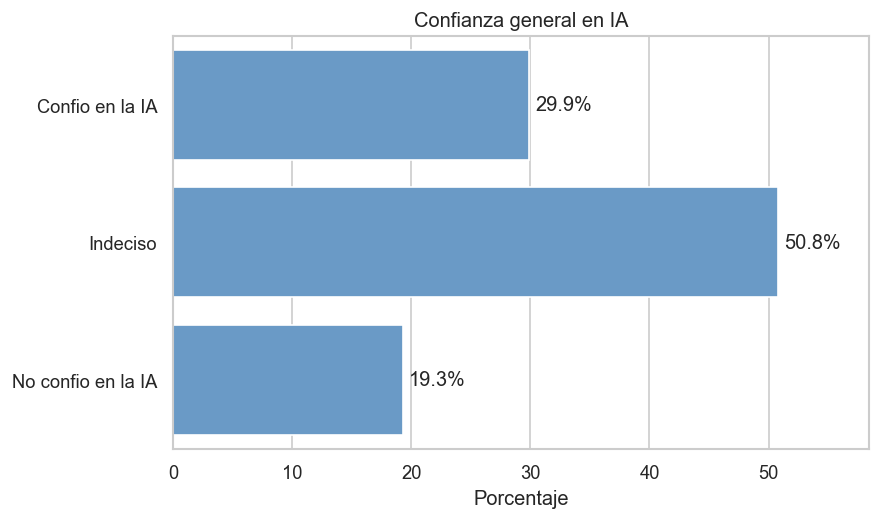
\includegraphics[width=\columnwidth]{graficos_informe/trust_ai.png}
\end{center}

Este gráfico responde a la pregunta: \textit{¿Qué percepciones de confianza y beneficio sobre la IA predominan en la sociedad?}

A partir del análisis de actitudes sociales (Data\_set\_02), se exploraron las visiones del público respecto a los riesgos y beneficios de la IA. La distribución evidencia una polarización en la sociedad: mientras un sector adopta la tecnología con entusiasmo, existe una proporción considerable de usuarios cautelosos. Esta falta de consenso sugiere que la adopción masiva y el éxito de estas herramientas dependerán en gran medida de las garantías de transparencia y seguridad que los desarrolladores logren comunicar al público.
\end{figure}

\begin{figure}[!htbp]
\textbf{Gráfico 2: Percepción de amenaza a libertades individuales}

\begin{center}
\includegraphics[width=\columnwidth]{graficos_informe/threat_freedoms.png}
\end{center}

Este gráfico responde a la pregunta: \textit{¿Cómo interactúa el nivel de confianza en la IA con la percepción de amenaza a las libertades individuales o el apoyo a regulaciones éticas?}

Como se observa, existe un debate importante frente a los riesgos potenciales. Una porción significativa de la muestra considera que la IA podría amenazar libertades individuales o requerir estrictas reglas éticas. Estos datos revelan un temor subyacente hacia la pérdida de autonomía y privacidad. La exigencia ciudadana por marcos éticos indica que el avance tecnológico debe ir necesariamente acompañado de políticas públicas sólidas, evitando que el desarrollo algorítmico vulnere los derechos individuales.
\end{figure}

\begin{figure}[!htbp]
\textbf{Gráfico 3: Relación entre confianza en IA y percepción de beneficio}

\begin{center}
\includegraphics[width=\columnwidth]{graficos_informe/trust_benefit_bar.png}
\end{center}

Este gráfico responde a la pregunta: \textit{¿De qué manera condiciona la confianza en la IA a la evaluación social de sus beneficios?}

El gráfico de barras evidencia claramente cómo la confianza condiciona la evaluación social de la herramienta: entre quienes confían en la IA, predomina ampliamente la percepción de que será "Más beneficiosa", mientras que en el grupo de quienes desconfían, la opinión mayoritaria es que será "Más dañina". Esta fuerte correlación demuestra que la percepción de utilidad no es puramente objetiva, sino que está filtrada por un sesgo previo. Por ende, cualquier estrategia para fomentar la IA debe enfocarse primero en generar credibilidad y educar tecnológicamente.
\end{figure}

\subsection*{Salud mental y reemplazo de tareas}
\textbf{Datos utilizados:} burnout\_score, job\_satisfaction\_1\_5, ai\_replaces\_my\_tasks\_pct y hours\_with\_ai\_assistance\_daily. Fuente: Data\_set\_01 [2].

\begin{figure*}[!htbp]
\textbf{Gráfico 4: Percepción de reemplazo por IA vs. nivel de agotamiento en roles frecuentes}

\vspace{0.2cm}
\begin{center}
\begin{minipage}{0.48\textwidth}
\centering
\includegraphics[width=\textwidth]{graficos_informe/ds03_reemplazo_burnout_software_engineer.png}\\
\scriptsize (a) Software Engineer.
\end{minipage}
\hfill
\begin{minipage}{0.48\textwidth}
\centering
\includegraphics[width=\textwidth]{graficos_informe/ds03_reemplazo_burnout_ai_researcher.png}\\
\scriptsize (b) AI Researcher.
\end{minipage}

\vspace{0.4cm}
\begin{minipage}{0.48\textwidth}
\centering
\includegraphics[width=\textwidth]{graficos_informe/ds03_reemplazo_burnout_data_scientist.png}\\
\scriptsize (c) Data Scientist.
\end{minipage}
\hfill
\begin{minipage}{0.48\textwidth}
\centering
\includegraphics[width=\textwidth]{graficos_informe/ds03_reemplazo_burnout_ai_ethics_officer.png}\\
\scriptsize (d) AI Ethics Officer.
\end{minipage}
\end{center}

Este gráfico responde a la pregunta: \textit{¿Cómo se asocian burnout, satisfacción laboral y reemplazo de tareas con la intensidad de uso de IA en el trabajo?}

En todos los casos se observa una tendencia positiva entre la percepción de reemplazo y el agotamiento. Este patrón es consistente con la literatura sobre riesgos y efectos sociales de los modelos de lenguaje en el trabajo [6-8]. La interpretación de estos datos sugiere que el miedo a la obsolescencia laboral genera una carga psicológica significativa (burnout). Independientemente del rol técnico, la incertidumbre sobre la estabilidad del empleo actúa como un estresor crónico que deteriora el bienestar y el clima organizacional.
\end{figure*}

\subsection*{Educación e impacto en el rendimiento}
\textbf{Datos utilizados:} rendimiento académico (final\_score), uso de IA (uses\_ai) y nivel de dependencia (ai\_dependency\_score). Fuente: Data\_set\_03 [1].

\begin{figure}[!htbp]
\textbf{Gráfico 5: Distribución del puntaje final comparando estudiantes que usan y no usan IA}

\begin{center}
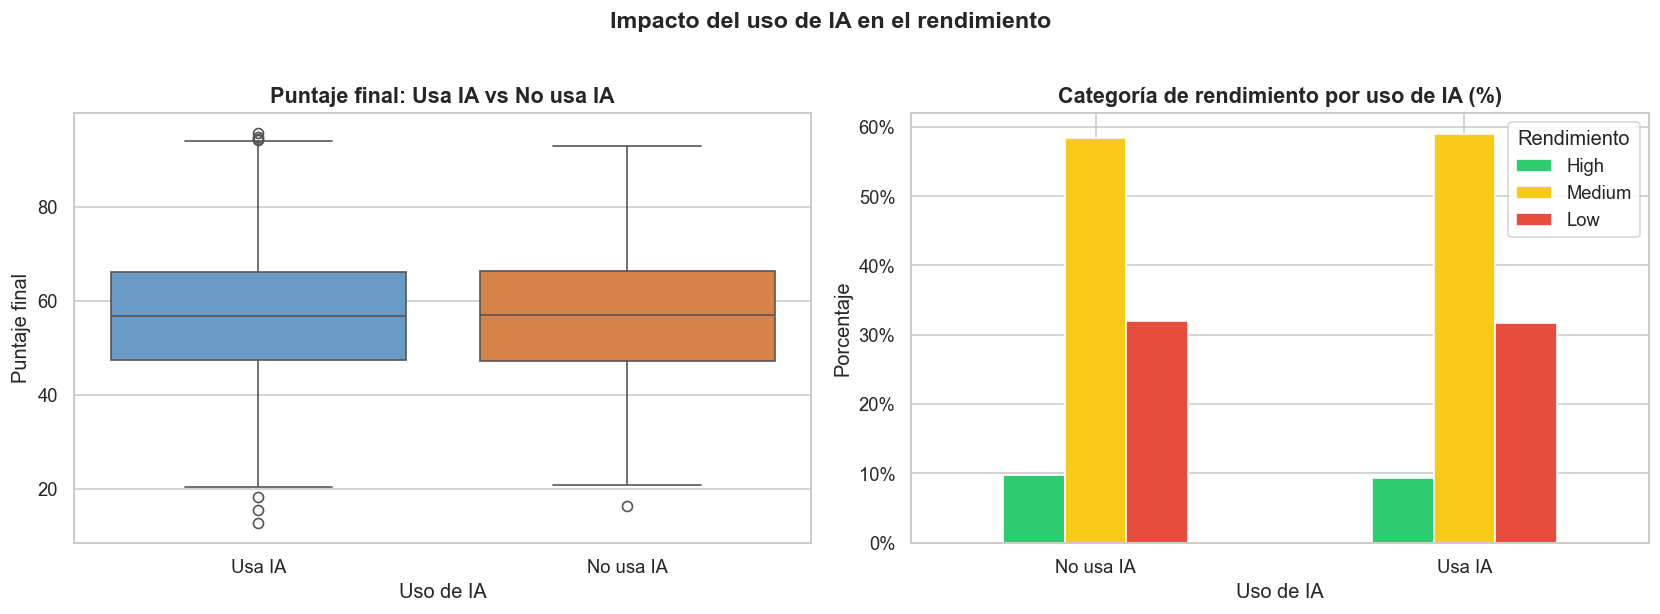
\includegraphics[width=\columnwidth]{graficos_informe/ds03_rendimiento_vs_ia.png}
\end{center}

Este gráfico responde a la pregunta: \textit{¿De qué manera incide el uso de IA en el rendimiento académico de los estudiantes?}

Utilizando el conjunto de datos enfocado en estudiantes (Data\_set\_03), se evaluó cómo el uso de la IA se relaciona con las calificaciones. La figura permite contrastar los resultados académicos entre ambos grupos, ofreciendo una primera aproximación a posibles beneficios o perjuicios. Los resultados sugieren que el mero acceso a la IA introduce diferencias en el rendimiento, pero no garantiza el éxito por sí solo. Esto abre el debate sobre la "brecha algorítmica", donde las habilidades de estructuración de \textit{prompts} se vuelven un nuevo factor diferenciador en las aulas.
\end{figure}

\begin{figure}[!htbp]
\textbf{Gráfico 6: Relación entre el puntaje final y el nivel de dependencia de la IA}

\begin{center}
\includegraphics[width=\columnwidth]{graficos_informe/ds03_dependencia_rendimiento.png}
\end{center}

Este gráfico responde a la pregunta: \textit{¿De qué manera incide el nivel de dependencia de IA en el rendimiento académico de los estudiantes?}

Al observar a los estudiantes que sí utilizan la IA, la relación entre su nivel de dependencia de la herramienta y sus calificaciones finales sugiere que un uso excesivo o no crítico podría asociarse a menores puntajes. La interpretación clave es que la IA debe actuar como un "copiloto" y no como un reemplazo del esfuerzo cognitivo. Delegar excesivamente la resolución de problemas en la inteligencia artificial parece atrofiar las habilidades analíticas propias del estudiante, lo que se traduce en un desempeño deficiente.
\end{figure}

\subsection*{Desarrollo Geográfico de la IA}
\textbf{Datos utilizados:} distribución geográfica y evolución de patentes de Inteligencia Artificial (2022-2024). Fuente: OCDE API.

\begin{figure}[!htbp]
\textbf{Gráfico 7: Distribución global de patentes de IA (2022-2024)}

\begin{center}

\includegraphics[width=\columnwidth]{Data/ocde_ia/mapa_patentes_ia_ocde_2022_2024.png}
\end{center}

Este gráfico responde a la pregunta: \textit{¿Cómo se distribuye geográficamente el desarrollo de Inteligencia Artificial?}

A partir de los datos recolectados de la API de la OCDE mediante el \textit{crawler}, se analizó el panorama global del desarrollo de la Inteligencia Artificial a través del registro de patentes. La concentración visual en el mapa subraya una marcada hegemonía tecnológica en regiones específicas del hemisferio norte. Este desbalance geográfico plantea riesgos de dependencia tecnológica para las naciones en desarrollo, las cuales actúan como consumidoras pasivas sin participar del diseño algorítmico y sus regulaciones.
\end{figure}

\begin{figure}[!htbp]
\textbf{Gráfico 8: Top 15 países en desarrollo de patentes de IA (2022-2024)}

\begin{center}
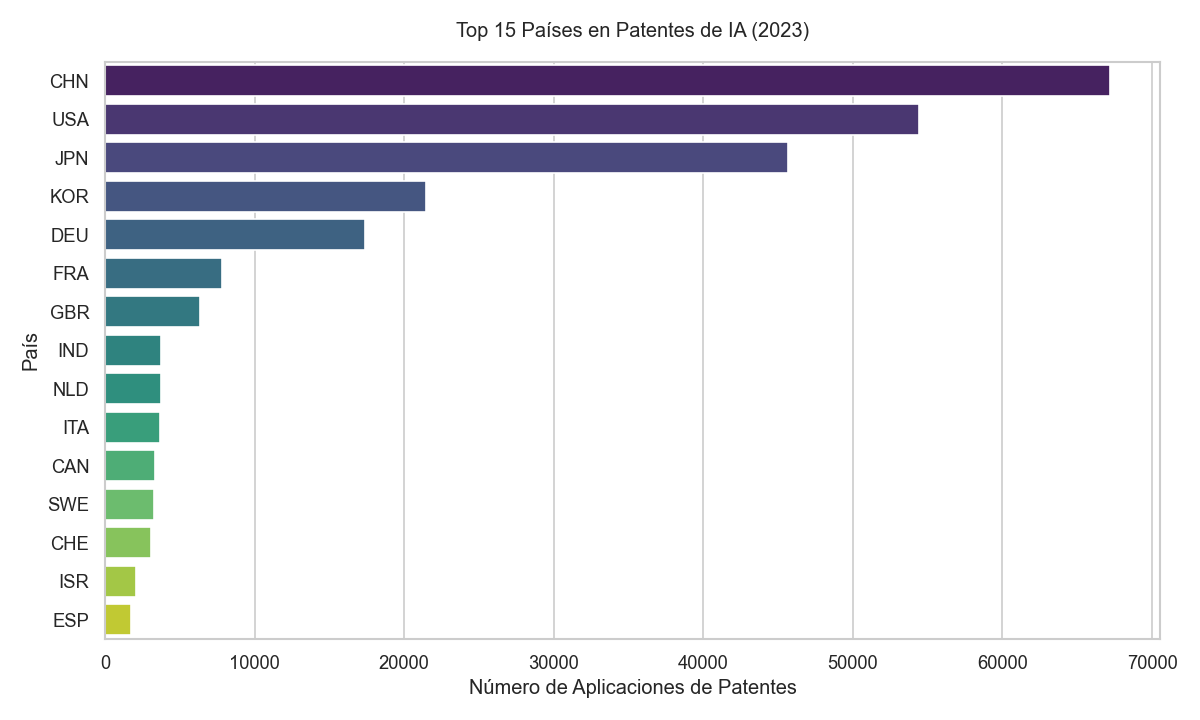
\includegraphics[width=\columnwidth]{graficos_api_ocde/top15_patentes_ia.png}
\end{center}

Este gráfico responde a la pregunta: \textit{¿Qué naciones lideran la adopción técnica e investigación en IA a nivel mundial?}

Estos gráficos permiten observar qué naciones lideran la adopción técnica e investigación en IA a nivel mundial, evidenciando los principales polos de desarrollo tecnológico. El ranking expone claramente la carrera internacional por el liderazgo en IA, comandada por países con robustos ecosistemas de investigación y alta inversión de capital (como EE. UU. y naciones asiáticas de primera línea). Esta aglomeración corporativa sugiere que los futuros estándares éticos y técnicos de la IA serán dictados por un grupo reducido de actores dominantes.
\end{figure}

\subsection*{Descripción breve de los datos analizados}
En esta etapa se usaron los conjuntos Data\_set\_01 (enfocado en Burnout y reemplazo de tareas), Data\_set\_02 (enfocado en percepciones sociales y riesgos de la IA), Data\_set\_03 (enfocado en el impacto de la IA en estudiantes), y datos recopilados de la OCDE. Los registros a nivel individual permitieron identificar contrastes importantes de actitudes frente a estas herramientas y analizar su efecto transversal en distintas áreas.
\subsection*{Vinculación con las preguntas de investigación}
Los resultados preliminares se conectan directamente con las preguntas planteadas en la introducción:
\begin{itemize}
\item \textbf{Pregunta 1:} relación entre reemplazo de tareas y agotamiento laboral por rol (Data\_set\_01).
\item \textbf{Preguntas 2 y 3:} distribución de actitudes sobre los beneficios de la IA y su interacción con las preocupaciones por libertades individuales (Data\_set\_02).
\item \textbf{Pregunta 4:} contraste de puntajes finales según uso y nivel de dependencia de la IA (Data\_set\_03).
\item \textbf{Pregunta 5:} distribución de patentes de Inteligencia Artificial para visualizar el liderazgo mundial en IA (Datos OCDE).
\end{itemize}


\clearpage
\section{Referencias bibliográficas}
\begin{enumerate}
    \item Mazari, A. \emph{Learning in the Age of AI: Myths and Facts} [Conjunto de datos]. Kaggle. Disponible en: \url{https://www.kaggle.com/code/abdullahmazari/learning-in-the-age-of-ai-myths-and-facts/input} (consulta: 01-05-2026).
    \item Justin, T. \emph{AI Worker Burnout 2026 - EDA} [Conjunto de datos]. Kaggle. Disponible en: \url{https://www.kaggle.com/code/tolstoyjustin/ai-worker-burnout-2026-eda/input} (consulta: 01-05-2026).
    \item uom190346a. \emph{AI-powered Job Market Insights} [Conjunto de datos]. Kaggle. Disponible en: \url{https://www.kaggle.com/datasets/uom190346a/ai-powered-job-market-insights} (consulta: 01-05-2026).
    \item Keskin, A. Y. \emph{The Impact of Artificial Intelligence on Society} [Conjunto de datos]. Kaggle. Disponible en: \url{https://www.kaggle.com/datasets/ardayavuzkeskin/the-impact-of-artificial-intelligence-on-society} (consulta: 01-05-2026).
    \item Geerling, W., Mateer, G. D., Wooten, J. y Damodaran, N. \emph{ChatGPT has Aced the Test of Understanding in College Economics: Now What?}. \emph{The American Economist}, 68(2) (2023). Disponible en: \url{https://journals.sagepub.com/doi/10.1177/05694345231169654}
    \item Weidinger, L., Mellor, J., Rauh, M., Griffin, C., Uesato, J., Huang, P.-S., et al. \emph{Ethical and social risks of harm from Language Models}. \emph{arXiv} (2021). Disponible en: \url{https://doi.org/10.48550/arXiv.2112.04359} (consulta: 01-05-2026).
    \item Eloundou, T., Manning, S., Mishkin, P. y Rock, D. \emph{GPTs are GPTs: An Early Look at the Labor Market Impact Potential of Large Language Models}. \emph{arXiv} (2023). Disponible en: \url{https://doi.org/10.48550/arXiv.2303.10130} (consulta: 01-05-2026).
    \item Brynjolfsson, E., Li, D. y Raymond, L. R. \emph{Generative AI at Work}. \emph{NBER Working Paper} 31161 (2023). Disponible en: \url{https://www.nber.org/papers/w31161} (consulta: 01-05-2026).
    \item World Economic Forum. \emph{The Future of Jobs Report 2023}. Disponible en: \url{https://www.weforum.org/reports/the-future-of-jobs-report-2023/} (consulta: 01-05-2026).
\end{enumerate}

\end{document}
